% !TEX root = ../vr_st.tex

\subsection{Real projective spaces}\label{s:first_critical_value_rpn}

Let us now focus on the real equatorial system with the antipodal action.
We will consider every sphere \(\bS^n(2)\) to have radius 2 so the quotient \(\rp^n\) has the same diameter as \(\bS^n\).
We will consider reduced (co)homology with mod 2 coefficients.

%Recall that $\bS^n(\rho)$ denotes the $n$-sphere of radius $\rho$ equipped with the geodesic distance $d$.
%The \defn{$n$-real projective space} $\rp^n(r)$ is the quotient space $\bS^n(r)$ by the antipodal map $x \mapsto -x$ for all $x \in \bS^n$.
%We equip $\rp^n(r)$ with the quotient metric.
% \[
% d\big([x],[x']\big) =
% \min\set[\big]{d(x, x'), d(-x, x')}.
% \]

%To simplify notation we denote $\bS(1)$ by $\bS^n$ and $\rp^n(2)$ by $\rp^n$.
%Notice that $\diam(\bS^n) = \diam(\rp^n) = \pi$.
%
%The inclusion of \(\mathbb{S}^n\) into \(\mathbb{S}^{n+1}\) as the equatorial $n$-sphere is equivariant with respect to the antipodal action.
%Therefore, it induces an inclusion of \(\rp^n\) into \(\rp^{n+1}\).

%Since the \defn{infinite sphere} \(\mathbb{S}^\infty = \bigcup_n \mathbb{S}^n\) is contractible, its induced projection onto the \defn{real projective space} $\rp^\infty = \bigcup_n \rp^n$ defines its universal cover, so $\rp^\infty$ is a model for \(K(\Z/2, 1)\).
%
%Consider the mod-\(2\) (co)homology of \(\VR(\rp^n)\) and the linear cohomology operations defined by Steenrod squares \(\Sq^k_\ell \in \cO(\ell,\ell+k)\).

%In certain intervals, the homotopy type of the Vietoris--Rips complex of $\rp^n$ is known.
%This information is presented in \cite[Thm.~4.5]{adams2022metric}:
%%\label{prop:RPn}{\rm \cite[Thm.~4.5]{adams2022metric}.}
%For $r \in (0,\frac{2\pi}{3} ]$,
%\[
%\VR_r(\rp^n) \simeq \rp^n,
%\]
%and the homotopy type of $\VR_r(\rp^n)$ changes after $\tfrac{2\pi}{3}$.
%In other words,

%\proposition
%%The first critical value of \(\VR(\rp^n)\) is
%For every \(n \in \N\),
%\[
%\crit(\rp^n) = \frac{2\pi}{3}.
%\]
%
%\begin{proof}
%	This proposition is stated and proven in \cite[Thm.~4.5]{adams2022metric}.
%\end{proof}

%We apply \cref{sub:general_barcodes} to prove the following proposition.

%\proposition
%For every \(m,n \in \N\),
%\[
%\firstdeath{m}{\rp^n} =
%\begin{cases}
%	\frac{\pi}{3} & 1 \leq m \leq n, \\
%	\hfil 0 & \text{otherwise}.
%\end{cases}
%\]
%
%\begin{proof}%[Proof of \cref{s:first_critical_value_rpn}.]
%	We only need to prove for the case of $1\leq m\leq n$, since the other case is follows from definition since \(\rH_m(\rp^n) = 0\) if \(m > n\) or \(m = 0\).
%    Recall from \cite{katz1983filling} that the filling radius of $\rp^n$ is $\frac{\pi}{3}$ for any $n \geq 1$.
%%	By considering the $\rC_2$-action on the equatorial system $\bS^m \to \bS^n$ and applying
%	By \cref{subsub:foundamental_bar_rpn_lemma}, we have that $\firstdeath{m}{\rp^n}\leq \tfrac{\pi}{3}$.
%    On the other hand, $\firstdeath{m}{\rp^n}\geq \tfrac{1}{2}\crit(\rp^n) = \tfrac{\pi}{3}$.
%\end{proof}

\medskip\proposition
For \(k,\ell,n,m \in \N\) and \(\Sq^k \in \cO(\ell, k+\ell)\) we have:
\begin{enumerate}
	\item \(\crit(\rp^n) = \frac{2\pi}{3}\).
	\item \(\firstdeath{m}{\rp^n} =
	\begin{cases}
		\frac{\pi}{3} & 1 \leq m \leq n, \\
		\hfil 0 & \text{otherwise}.
	\end{cases}\)
	\item \(\firstdeath{\Sq^k}{\rp^n} =
	\begin{cases}
		\tfrac{\pi}{3} & k \leq \frac{n-1}{2} \text{ and } \binom{\ell}{k} \text{ is odd},\\
		\hfil 0 & \text{otherwise}. \\
	\end{cases}\)
\end{enumerate}
%\[
%\firstdeath{\Sq^k}{\rp^n} =
%\begin{cases}
%	\tfrac{\pi}{3} & k \leq \frac{n-1}{2} \text{ and } \binom{\ell}{k} \text{ is odd},\\
%	\hfil 0 & \text{otherwise}. \\
%\end{cases}
%\]


\begin{proof}
	(1) This proposition is stated and proven in \cite[Thm.~4.5]{adams2022metric}.

	(2) We only need to prove for the case of $1\leq m\leq n$, since the other case is follows from definition since \(\rH_m(\rp^n) = 0\) if \(m > n\) or \(m = 0\).
	Recall from \cite{katz1983filling} that the filling radius of $\rp^n$ is $\frac{\pi}{3}$ for any $n \geq 1$.
	%	By considering the $\rC_2$-action on the equatorial system $\bS^m \to \bS^n$ and applying
	By \cref{subsub:foundamental_bar_rpn_lemma}, we have that $\firstdeath{m}{\rp^n}\leq \tfrac{\pi}{3}$.
	On the other hand, $\firstdeath{m}{\rp^n}\geq \tfrac{1}{2}\crit(\rp^n) = \tfrac{\pi}{3}$.

	(3) We only need a proof for the case $k \leq \frac{n-1}{2}$ and $\binom{\ell}{k}$ odd, since \(\Sq^k = 0\) otherwise.
    Given that $\VR_r(\rp^n)$ retains the homotopy type of $\rp^n$ for $r \in [0,\tfrac{2\pi}{3})$, \anibal{Recall the cohomology ring in order to use the generator \(\sigma\)} and $\Sq^k(\sigma^\ell) = \binom{\ell}{k}\sigma^{\ell+k}$ generates a bar in $\barc \img_{\Sq^k}$ that is born at $0$ and stays alive until the non-trivial degree-$(\ell+k)$ class $\sigma^{k+\ell}$ dies at $\tfrac{2\pi}{3}$.
	Thus, $\firstdeath{\Sq_\ell^k}{\rp^n} \leq \tfrac{\pi}{3}$.
	On the other hand, $\firstdeath{\Sq^k}{\rp^n} \geq \tfrac{1}{2}\crit(\rp^n) = \tfrac{\pi}{3}$.
\end{proof}

%We combine results in \cref{s:first_critical_value_rpn}, \cref{s:first_critical_value_rpn} and \cref{s:first_critical_value_rpn} with the barcode estimates in \cref{ss:barcode_general} to derive an estimate for the barcodes of $\rp^n$.
Using the above values, the estimates resulting from the analysis of \cref{ss:barcode_general} are illustrated in \cref{fig:sq barcodes}.

\begin{figure}
	\centering
	\begin{tikzpicture}[scale=0.52]
	\begin{axis} [
		title = {\LARGE $\Hbarc{\degp}{\rp^n},\, \degp\leq n$},
		ticklabel style = {font=\Large},
		axis y line=middle,
		axis x line=middle,
		ytick={0.5,0.67,0.95},
		yticklabels={$\frac{\pi}{2}$,$\frac{2\pi}{3}$,$\pi$},
		xtick={0.5,0.67,0.95},
		xticklabels={$\frac{\pi}{2}$,$\frac{2\pi}{3}$,$\pi$},
		xmin=-0.015, xmax=1.1,
		ymin=0, ymax=1.1,]
		\addplot [mark=none] coordinates {(0,0) (1,1)};
		\addplot [thick,color=black!20!white,fill=black!30!white,
		fill opacity=0.4]coordinates {
			(0.67,0.95)
			(0.67,0.67)
			(0.95,0.95)
			(0.67,0.95)};
		\addplot [black!40!white,mark=none,dashed, thin] coordinates {(0,0.67) (0.67,0.67)};
		%\addplot [black!40!white,mark=none,dashed, thin] coordinates {(0,0.72) (0.72,0.72)};
		\addplot [black!40!white,mark=none,dashed, thin] coordinates {(0.67,0) (0.67,0.67)};
		\addplot[barccolor,mark=*] (0, 0.67) circle (2pt) node[above right,barccolor]{};%{\Large\textsf{1}};
		%\node[mark=none] at (axis cs:0.68,0.21){$\Hbarc{1}{\rp^n}$};
	\end{axis}
\end{tikzpicture}
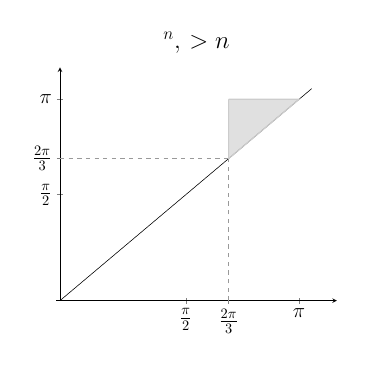
\begin{tikzpicture}[scale=0.52]
	\begin{axis} [
		title={\LARGE $\Hbarc{\degp}{\rp^n},\, \degp>n$},
		ticklabel style = {font=\Large},
		axis y line=middle,
		axis x line=middle,
		ytick={0.5,0.67,0.95},
		yticklabels={$\frac{\pi}{2}$,$\frac{2\pi}{3}$,$\pi$},
		xtick={0.5,0.67,0.95},
		xticklabels={$\frac{\pi}{2}$,$\frac{2\pi}{3}$,$\pi$},
		xmin=-0.015, xmax=1.1,
		ymin=0, ymax=1.1,]
		\addplot [mark=none] coordinates {(0,0) (1,1)};
		\addplot [thick,color=black!20!white,fill=black!30!white,
		fill opacity=0.4]coordinates {
			(0.67,0.95)
			(0.67,0.67)
			(0.95,0.95)
			(0.67,0.95)};
		\addplot [black!40!white,mark=none,dashed, thin] coordinates {(0,0.67) (0.67,0.67)};
		\addplot [black!40!white,mark=none,dashed, thin] coordinates {(0.67,0) (0.67,0.67)};
		% \addplot[barccolor,mark=*] (0, 0.67) circle (2pt) node[above right,barccolor]{\Large\textsf{1}};
		% \node[mark=none] at (axis cs:0.68,0.21){$\Hbarc{\degp}{\rp^n},\, \degp\geq 2$};
	\end{axis}
\end{tikzpicture}

\begin{tikzpicture}[scale=0.52]
	\begin{axis} [
		title = {\LARGE $\sqbarcl{k}{}{\rp^n},\, m \leq n$ and $\binom{m-k}{k}$ odd},
		ticklabel style = {font=\Large},
		axis y line=middle,
		axis x line=middle,
		ytick={0.5,0.67,0.95},
		yticklabels={$\frac{\pi}{2}$,$\frac{2\pi}{3}$,$\pi$},
		xtick={0.5,0.67,0.95},
		xticklabels={$\frac{\pi}{2}$,$\frac{2\pi}{3}$,$\pi$},
		xmin=-0.015, xmax=1.1,
		ymin=0, ymax=1.1,]
		\addplot [mark=none] coordinates {(0,0) (1,1)};
		\addplot [thick,color=black!20!white,fill=black!30!white,
		fill opacity=0.4]coordinates {
			(0.67,0.95)
			(0.67,0.67)
			(0.95,0.95)
			(0.67,0.95)};
		\addplot [black!40!white,mark=none,dashed, thin] coordinates {(0,0.67) (0.67,0.67)};
		%\addplot [black!40!white,mark=none,dashed, thin] coordinates {(0,0.72) (0.72,0.72)};
		\addplot [black!40!white,mark=none,dashed, thin] coordinates {(0.67,0) (0.67,0.67)};
		\addplot[barccolor,mark=*] (0, 0.67) circle (2pt) node[above right,barccolor]{};
        %{\Large$\geq$\textsf{1}};
	\end{axis}
\end{tikzpicture}
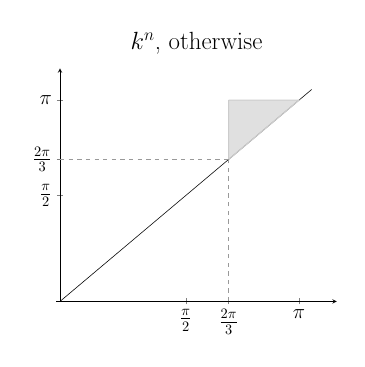
\begin{tikzpicture}[scale=0.52]
	\begin{axis} [
		title={\LARGE $\sqbarcl{k}{}{\rp^n}$, otherwise},
		ticklabel style = {font=\Large},
		axis y line=middle,
		axis x line=middle,
		ytick={0.5,0.67,0.95},
		yticklabels={$\frac{\pi}{2}$,$\frac{2\pi}{3}$,$\pi$},
		xtick={0.5,0.67,0.95},
		xticklabels={$\frac{\pi}{2}$,$\frac{2\pi}{3}$,$\pi$},
		xmin=-0.015, xmax=1.1,
		ymin=0, ymax=1.1,]
		\addplot [mark=none] coordinates {(0,0) (1,1)};
		\addplot [thick,color=black!20!white,fill=black!30!white,
		fill opacity=0.4]coordinates {
			(0.67,0.95)
			(0.67,0.67)
			(0.95,0.95)
			(0.67,0.95)};
		\addplot [black!40!white,mark=none,dashed, thin] coordinates {(0,0.67) (0.67,0.67)};
		\addplot [black!40!white,mark=none,dashed, thin] coordinates {(0.67,0) (0.67,0.67)};
	\end{axis}
\end{tikzpicture}
	\caption{\emph{Top row:} the persistent reduced homology barcode of $\rp^n$.
		%When $1\leq \degp \leq n$, the barcode consists of one $(0,\frac{2\pi}{3})$ and potentially some bars dominated by $(\frac{2\pi}{3}, \pi)$.
		\emph{Bottom row:} the $\img_{\Sq_\ell^k}$-barcode of $\rp^n$.
		%The leftmost barcode contains at least one $(0,\frac{2\pi}{3})$ and potentially some bars dominated by $(\frac{2\pi}{3}, \pi)$;
        %See \cref{s:first_critical_value_rpn} for details.
        In each figure, the gray region represents where additional bars could exist within the corresponding barcode.
	}
	\label{fig:sq barcodes}
\end{figure}
